Evaluation of ESN performance on the NARMA system is a thoroughly explored area
in the field of RC \cite{verstraeten_experimental_2007, rodan_minimum_2011,
jaeger_adaptive_nodate}. Similar performance to previous work has been achieved
(Fig. \ref{visualization}, \ref{performance}) as a baseline to lend credibility
to further approaches in this paper.

\begin{figure}[H]
  \centering
  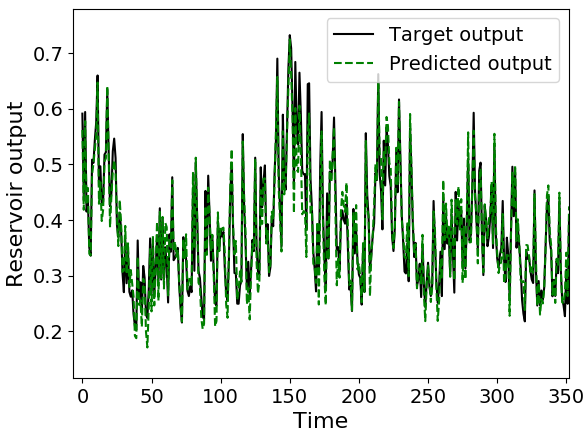
\includegraphics[width=2.5in]{img/narma_visualization.png}
  \caption{
    Visualization of reservoir output when fed the NARMA10 task. Input is an
i.i.d. stream generated uniformly in the interval [0, 0.5].
  }
  \label{visualization}
\end{figure}

\begin{figure}[H]
  \centering
  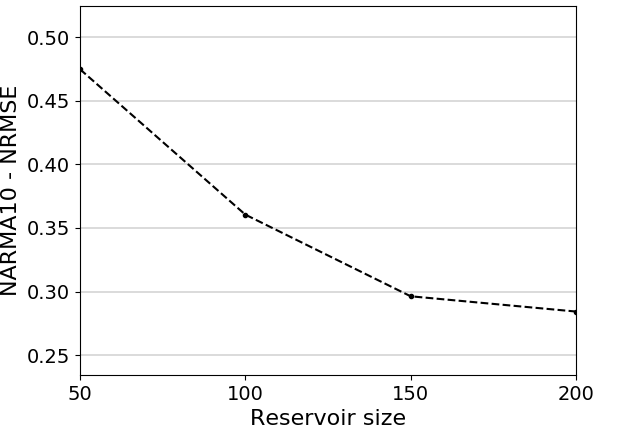
\includegraphics[width=2.5in]{img/general_performance.png}
  \caption{
    Reservoir size versus ESN performance for the NARMA10 task. The NRMSE is
averaged over 10 simulation runs.
  }
  \label{performance}
\end{figure}

All further reservoirs were constructed with the parameters from this baseline:
$\mathbf{W}^{res}$ and $\mathbf{W}^{in}$ were both generated as random matrices
with i.i.d. entries in the interval [-0.5, 0.5]. Both matrices are fully
connected, and the reservoir weight matrix was rescaled to have a spectral
radius of 0.9.

\begin{figure}[H]
  \centering
  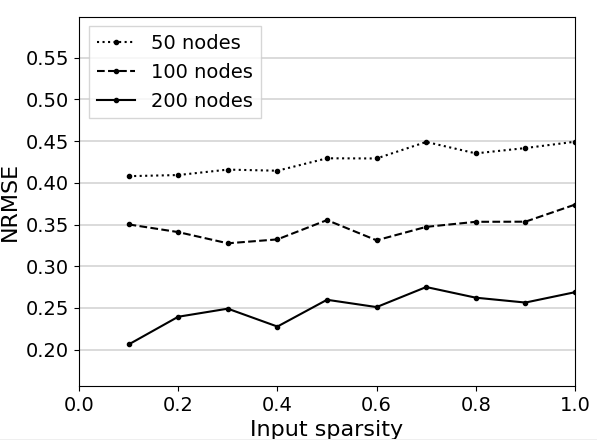
\includegraphics[width=2.5in]{img/input_sparsity_all.png}
  \caption{
    Input sparsity versus NRMSE for three different reservoir sizes.
  }
  \label{performance}
\end{figure}

\subsection{Noise}

\subsection{Measurement equipment accuracy}

\subsection{Partially visible state}

\subsection{Topology}


% Thoughts
% * Remember to add NRMSE to heatmap plots.

%%% Local Variables:
%%% mode: latex
%%% TeX-master: "../main"
%%% End:
